%!TEX program = xelatex
\documentclass[11pt,a4paper]{article}

% --- fonts / Chinese ---
\usepackage[UTF8,scheme=chinese]{ctex}
\usepackage{fontspec}
\setmainfont{TeX Gyre Termes}
\setmonofont{Latin Modern Mono}[Scale=0.92]

% --- core ---
\usepackage{amsmath,amssymb,bm}
\usepackage{booktabs,tabularx,array,multirow}
\usepackage{graphicx}
\usepackage{subcaption}
\usepackage{float}
\usepackage{natbib}
\usepackage{xcolor}
\usepackage[margin=2.5cm]{geometry}
\usepackage{hyperref}
\usepackage{setspace}
\onehalfspacing
\usepackage{caption}
\captionsetup{font=small,labelfont=bf,skip=6pt}

\hypersetup{colorlinks=true,linkcolor=black,citecolor=black,urlcolor=black}

\newcolumntype{L}{>{\raggedright\arraybackslash}X}
\newcolumntype{C}{>{\centering\arraybackslash}X}

\title{G1 运动控制 (AI 翻译版,原版为 report.pdf)}
\author{
  \begin{tabular}{c}
    李子墨 \\
    \small 学号 241098038 \\
    \small \texttt{3234454007@qq.com}
  \end{tabular}
}
\date{}

\begin{document}
\maketitle

\begin{abstract}

我使用 PPO 为宇树 G1 人形机器人训练了速度跟踪策略，并在此基础上实现了目标点跟踪。
此外，我针对策略的两类分布外（OOD）场景——OOD 速度与 OOD 地形——进行了实验，并通过微调克服了相应的失败。

\end{abstract}

\section{引言}

目标是在 Isaac Lab 中让宇树 G1 走到指定目标点。我分两步完成。

\textbf{训练：} 使用 PPO 训练速度跟踪策略。其指令为
$(v_x,v_y,\omega_z)$，其中 $v_x$ 为前进速度，$v_y$ 为侧向速度，
$\omega_z$ 为转向角速度。

\textbf{推理：} 固定已训练策略。用简单的比例控制器将相对目标位置
转换为速度指令，策略再跟踪该指令以到达目标。

我还在两类超出训练分布的情形下测试策略：
\begin{itemize}
  \item \textbf{更快指令：} 基础策略在
  $v_x\in[0,1]\,\mathrm{m/s}$ 下训练，测试时速度最高至
  $2\,\mathrm{m/s}$。
  \item \textbf{崎岖地形：} 将平地策略在楼梯、箱子、斜坡与高度噪声等
  地形上测试并微调。
\end{itemize}

在录制测试中，基础策略在
$v_x=1.4\,\mathrm{m/s}$ 时跌倒，而微调后的策略可在
$2\,\mathrm{m/s}$ 下行走。经短暂的崎岖地形微调后，策略也能在无高度扫描的
情况下走过所测的不规则地面。

\section{相关工作}
\label{sec:related}

\paragraph{双足运动。}
经典双足控制器常借助 SLIP~\citep{blickhan1989slip}、LIP~\citep{kajita2001lip}、
ZMP~\citep{vukobratovic2004zmp} 等简化模型规划稳定运动。这类方法直接建模平衡，
但需要精心设计的控制器。

\paragraph{学习运动。}
深度强化学习可直接从仿真经验中学习运动。借助数千个并行环境，
速度跟踪策略可被高效训练~\citep{rudin2022legged}。
我沿用该方法训练 G1。

\paragraph{训练工具。}
PPO 是一种 actor--critic 算法，通过裁剪目标限制每次策略更新幅度~\citep{schulman2017ppo}。
我使用 RSL-RL 中的 PPO、Isaac Sim 的 GPU 并行物理，以及 Isaac Lab 中的
G1 机器人与运动环境。

\section{训练}
\label{sec:train}

我在 Isaac Lab 中仿真宇树 G1，并用 PPO（RSL-RL）训练速度跟踪策略。
4096 个环境在 GPU 上并行运行；每一步策略输出关节目标，物理仿真推进，并收集奖励用于更新。
策略跟踪随机采样的指令 $\mathbf{c}_t = (v_x, v_y, \omega_z)$。

\subsection{MDP}

学习目标是使 G1 跟随指令平面速度
$\mathbf{c}_t=(v_x,v_y,\omega_z)$。我使用官方平地任务
\texttt{G1FlatEnvCfg}，并关闭其高度扫描仪。一个控制步流程如下：策略观测机器人与当前指令，
为每个主动关节输出目标偏移；随后仿真器推进物理，并评估运动对指令的跟踪效果。

形式上，仿真器状态 $s_t$ 包含机器人与环境的完整物理状态。策略并不直接接收 $s_t$，
而是接收 123 维观测
\[
\mathbf{o}_t =
\left[
\mathbf{v}^{b}_t,\,
\boldsymbol{\omega}^{b}_t,\,
\mathbf{g}^{b}_t,\,
\mathbf{c}_t,\,
\mathbf{q}_t-\mathbf{q}_{0},\,
\dot{\mathbf{q}}_t,\,
\mathbf{a}_{t-1}
\right],
\qquad \mathbf{o}_t\in\mathbb{R}^{123}.
\]
其中，$\mathbf{v}^{b}_t$ 与 $\boldsymbol{\omega}^{b}_t$ 分别为基座线速度与角速度
（各 3 维），$\mathbf{g}^{b}_t$ 为基座坐标系下的重力方向（3 维），$\mathbf{c}_t$ 为速度指令（3 维）。
其余项为相对默认姿态的 37 个关节位置、37 个关节速度，以及上一时刻的 37 维动作。
维度合计 $3+3+3+3+37+37+37=123$。训练时对机体与关节测量加入小幅均匀噪声。
由于关闭了高度扫描仪，策略无法直接获得地形描述。

\paragraph{动作与转移。}
动作 $\mathbf{a}_t\in\mathbb{R}^{37}$ 并不直接指定关节力矩，
而是相对默认姿态的位置偏移：
\[
\mathbf{q}^{\mathrm{target}}_t
=\mathbf{q}_{0}+0.5\,\mathbf{a}_t.
\]
关节控制器跟踪这些目标，同时 Isaac Sim 将机器人动力学从 $s_t$ 推进到 $s_{t+1}$。
将 $\mathbf{a}_{t-1}$ 纳入下一步观测，使策略在生成平滑动作序列时能考虑上一目标。

\paragraph{奖励与终止。}
奖励为官方 G1 平地任务给出的加权和。最大的正向项奖励跟踪指令 XY 速度与偏航角速度
（权重各 $+1.0$）。足部腾空时间项（$+0.75$）鼓励迈步。
惩罚项抑制足部滑动（$-0.1$）、身体倾斜（$-1.0$）、竖直速度（$-0.2$）、
滚转与俯仰角速度（$-0.05$），以及关节偏离或越限（权重从 $-1.0$ 到 $-0.05$）。
较小的正则项惩罚动作剧烈变化（$-5{\times}10^{-3}$）、关节力矩（$-2{\times}10^{-6}$）
与关节加速度（$-1{\times}10^{-7}$）。终止时奖励为 $-200$。
因此，最大化回报要求机器人跟随指令，同时保持稳定、平滑且物理上合理的步态。

\paragraph{PPO 配置。}
Actor 与 critic 使用隐藏层为 $[256,128,128]$ 的 MLP。PPO 每次迭代从 4096 个并行环境
各采集 24 步，裁剪参数 $0.2$，折扣因子 $\gamma=0.99$，GAE 参数 $\lambda=0.95$，
熵系数 $0.008$。

\subsection{速度策略训练}

我训练一个策略，使其在平地上跟随随机采样的速度指令。指令范围为
\[
v_x \in [0, 1]\,\mathrm{m/s},\quad
v_y \in [-0.5, 0.5]\,\mathrm{m/s},\quad
\omega_z \in [-1, 1]\,\mathrm{rad/s},
\]
其中 $v_x$ 控制前进，$v_y$ 控制侧向，$\omega_z$ 控制转向。少量环境收到站立指令
$\mathbf{c}_t=\mathbf{0}$，因此同一策略也学会保持静止。训练共 1750 次迭代。
图~\ref{fig:tb-base} 显示平均奖励稳步上升、速度跟踪误差下降；
图~\ref{fig:train} 展示平地上的步态结果。

\begin{figure}[H]
\centering
\begin{subfigure}[t]{0.33\textwidth}
\centering
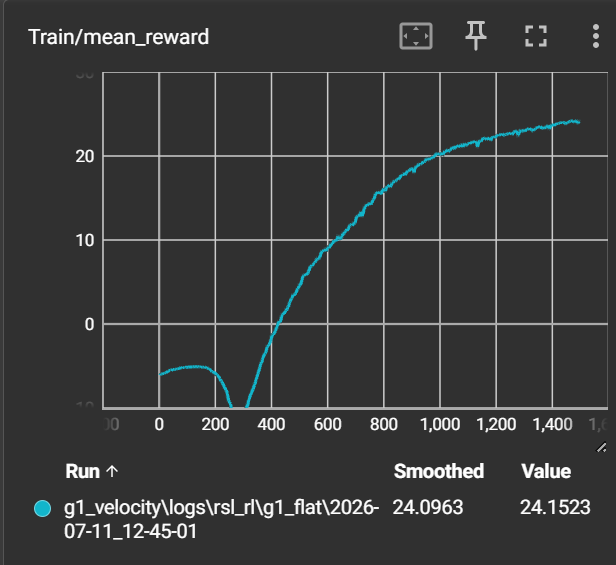
\includegraphics[width=\linewidth]{figures/tb-g1_velocity_mean_reward.png}
\caption*{平均奖励。}
\end{subfigure}
\hfill
\begin{subfigure}[t]{0.66\textwidth}
\centering
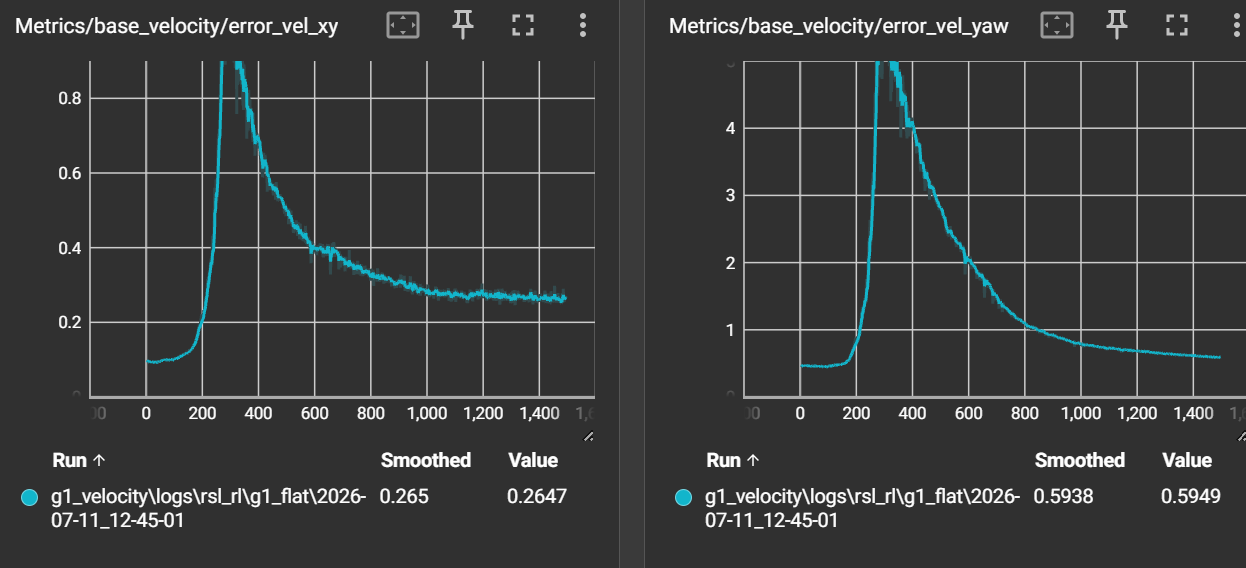
\includegraphics[width=\linewidth]{figures/tb_g1_velocity_metrics_error.png}
\caption*{速度跟踪误差。}
\end{subfigure}
\caption{基础速度策略训练曲线。}
\label{fig:tb-base}
\end{figure}

\begin{figure}[H]
\centering
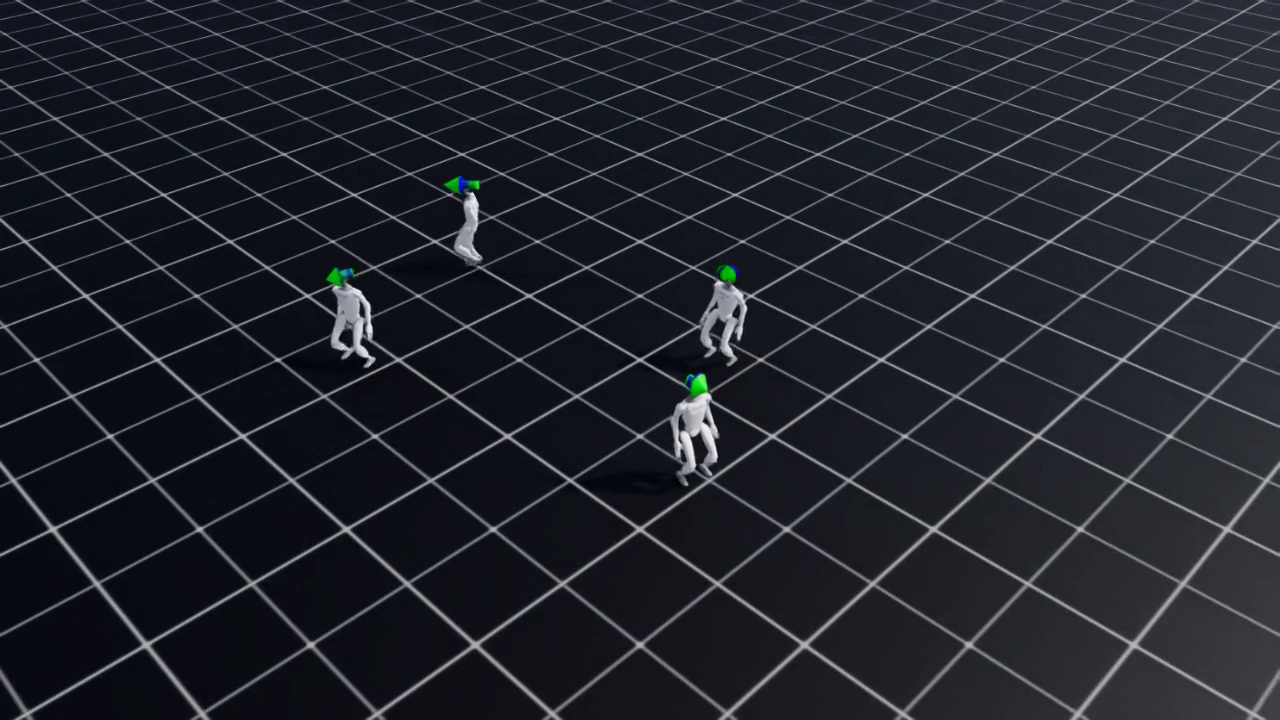
\includegraphics[width=0.72\textwidth]{figures/fig_flat.png}
\caption{训练得到的速度跟踪策略在平地上（随机指令）。}
\label{fig:train}
\end{figure}

\section{推理}
\label{sec:inference}

推理时固定策略权重，用比例控制器将目标位移转换为 $(v_x,v_y,\omega_z)$。
策略以与训练相同的观测与动作空间跟踪这些指令。

\paragraph{目标到速度的控制器。}
每个控制步，将世界坐标系下的目标表示到机器人偏航坐标系中为 $(d_x,d_y)$。角度
$\psi=\mathrm{atan2}(d_y,d_x)$ 为该坐标系下机器人到目标的方向。速度指令按如下计算：
\begin{enumerate}
  \item 若 $\sqrt{d_x^2+d_y^2}<0.35\,\mathrm{m}$，令
  $\mathbf{c}_t=\mathbf{0}$，使机器人在目标附近站立。
  \item 否则，施加比例控制：
  \[
  v_x = \mathrm{clip}(k_\ell d_x,\, 0,\, 1),\quad
  v_y = \mathrm{clip}(k_\ell d_y,\, -0.5,\, 0.5),\quad
  \omega_z = \mathrm{clip}(k_a \psi,\, -1,\, 1),
  \]
  其中 $k_\ell = 1.0$，$k_a = 1.5$。
\end{enumerate}
裁剪使每条指令落在训练所见范围内。特别地，控制器从不请求后退；当目标在机器人后方时，
偏航控制先转向目标，再发出明显的前进指令。

\paragraph{结果。}
在录制仿真中，冻结策略走向标记目标，并在进入 $0.35\,\mathrm{m}$ 停止区域后站立
（图~\ref{fig:inference}）。

\begin{figure}[H]
\centering
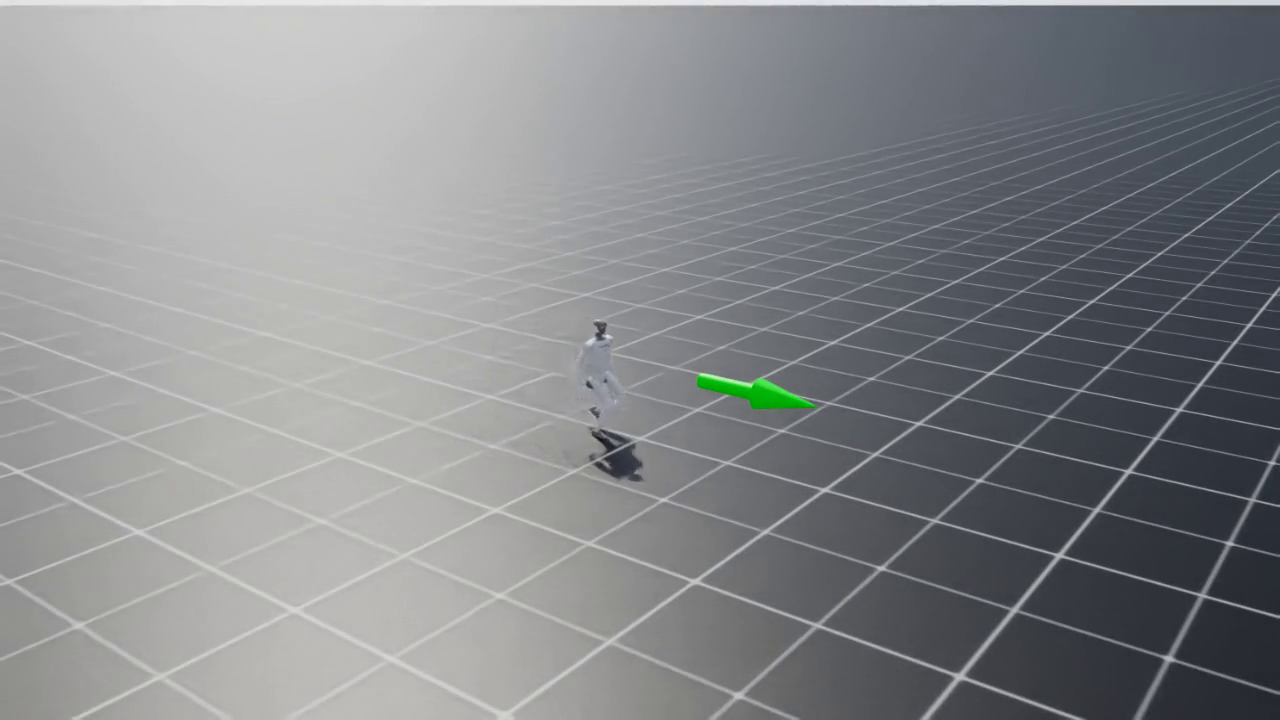
\includegraphics[width=0.72\textwidth]{figures/fig_goal.png}
\caption{目标导向推理。比例控制器引导冻结的速度策略走向绿色标记。}
\label{fig:inference}
\end{figure}

\section{探索实验一：前进速度泛化}
\label{sec:ood}

基础策略训练时前进指令不超过 $1\,\mathrm{m/s}$。本实验考察其收到更快指令时的表现，
以及微调能否扩展可用速度范围。机器人、地形、观测与动作保持不变；仅前进指令幅值
超出原训练分布。

\subsection{微调}

宽 $v_x$ 策略由基础策略初始化，并在前进指令最高 $2\,\mathrm{m/s}$ 下微调；
网络结构与目标控制器保持不变。侧向与偏航指令范围收窄，以强调前进运动：

\begin{table}[H]
\centering
\small
\begin{tabular}{@{}llll@{}}
\toprule
策略 & $v_x$ (m/s) & $v_y$ (m/s) & $\omega_z$ (rad/s) \\
\midrule
基础 & $[0,1]$ & $[-0.5,0.5]$ & $[-1,1]$ \\
宽 $v_x$ & $[0,2]$ & $[-0.2,0.2]$ & $[-0.5,0.5]$ \\
\bottomrule
\end{tabular}
\caption{训练两种策略所用的指令分布。}
\label{tab:ood-pol}
\end{table}

该指令分布使微调聚焦于前进运动。
图~\ref{fig:tb-wide} 显示平均奖励回升，速度跟踪误差下降。

\begin{figure}[H]
\centering
\begin{subfigure}[t]{0.33\textwidth}
\centering
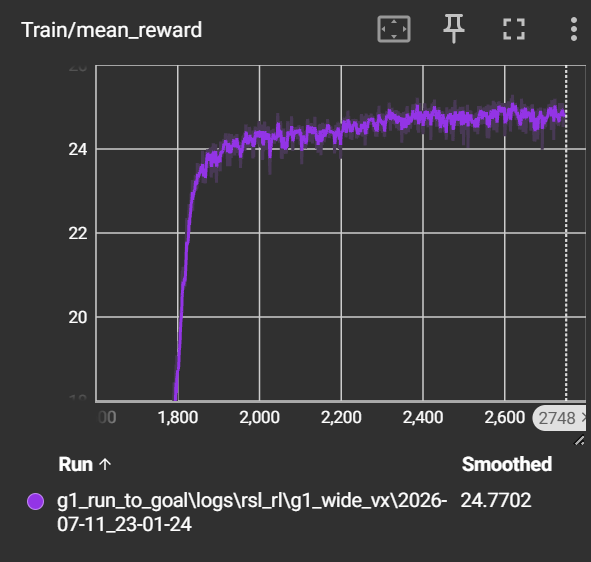
\includegraphics[width=\linewidth]{figures/tb_g1_wide_vx_mean_reward.png}
\caption*{平均奖励。}
\end{subfigure}
\hfill
\begin{subfigure}[t]{0.66\textwidth}
\centering
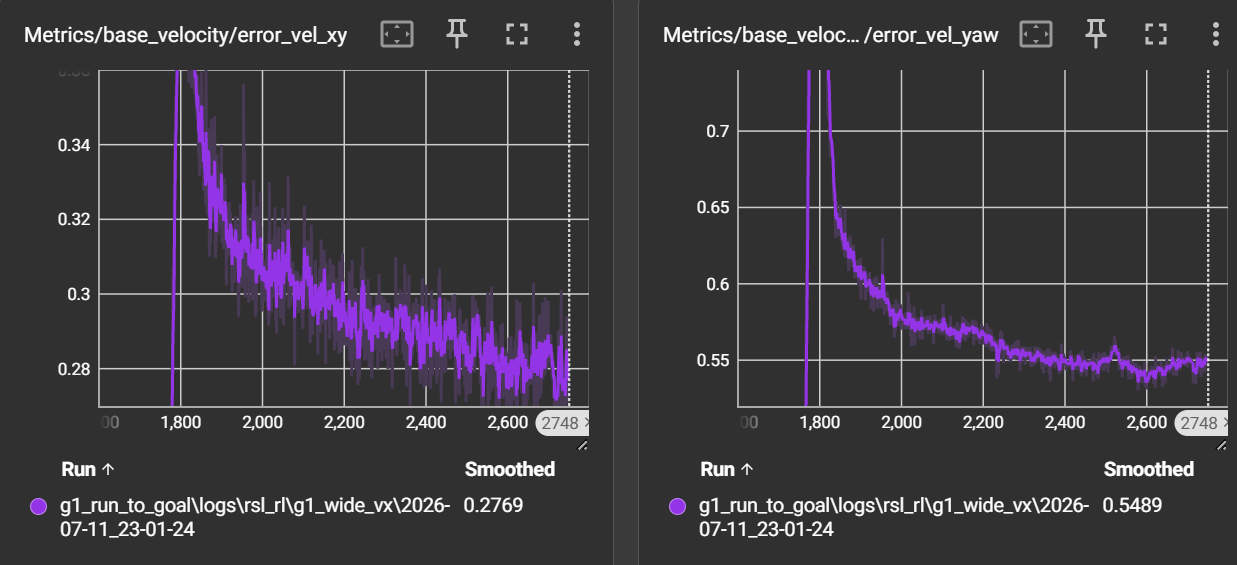
\includegraphics[width=\linewidth]{figures/tb_g1_wide_vx_metrics_error.png}
\caption*{速度跟踪误差。}
\end{subfigure}
\caption{宽 $v_x$ 微调曲线。}
\label{fig:tb-wide}
\end{figure}

\subsection{评估协议}

两种策略均接收固定、纯前进指令 $\mathbf{c}=(v_x,0,0)$。扫描覆盖
$0.2$ 至 $2.0\,\mathrm{m/s}$；不超过 $1.0\,\mathrm{m/s}$ 的指令对基础策略为分布内，
$1.1$ 至 $2.0\,\mathrm{m/s}$ 为分布外。关闭自动航向指令与站立环境，
使受测变量仅为指令前进速度。

我在每个速度下录制仿真片段，比较机器人是否保持直立并跟随指令。

\subsection{观测结果}

在录制扫描中，基础策略在 $v_x=1.3\,\mathrm{m/s}$ 时仍能直立，
但在 $1.4\,\mathrm{m/s}$ 及更高测试指令下跌倒。微调后，宽 $v_x$ 策略
在直至 $2.0\,\mathrm{m/s}$ 时仍保持直立并跟随前进指令。因此，微调将所测指令范围
扩展到超出基础策略。

\begin{figure}[H]
\centering
\begin{subfigure}[t]{0.48\textwidth}
\centering
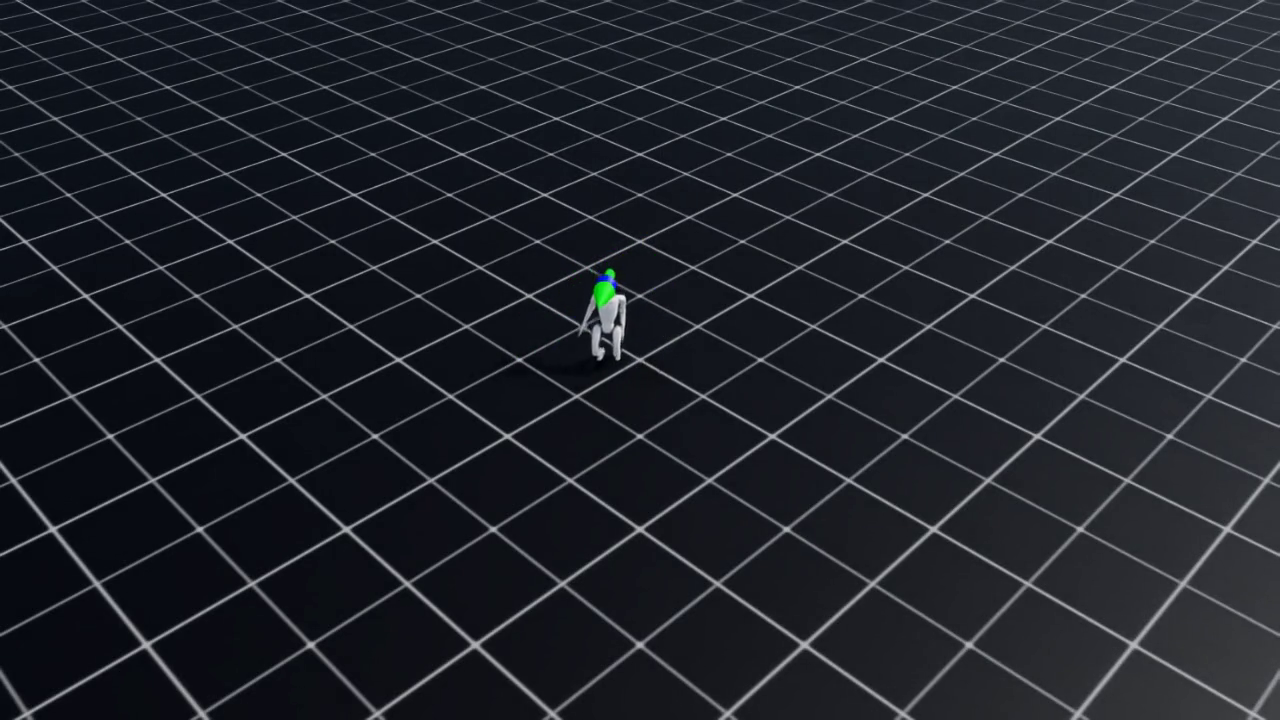
\includegraphics[width=\linewidth]{figures/fig_ood13.png}
\caption*{基础，$v_x{=}1.3\,\mathrm{m/s}$（稳定）。}
\end{subfigure}
\hfill
\begin{subfigure}[t]{0.48\textwidth}
\centering
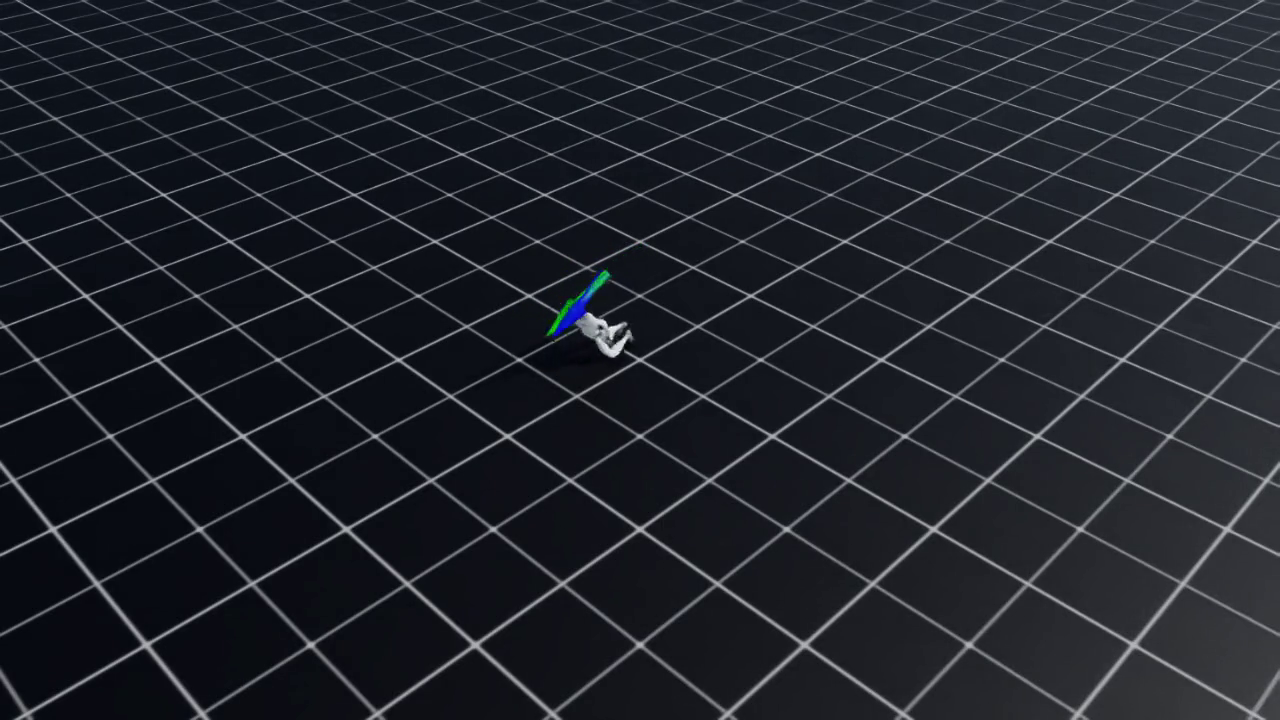
\includegraphics[width=\linewidth]{figures/fig_ood14.png}
\caption*{基础，$v_x{=}1.4\,\mathrm{m/s}$（跌倒）。}
\end{subfigure}

\vspace{0.6em}

\begin{subfigure}[t]{0.48\textwidth}
\centering
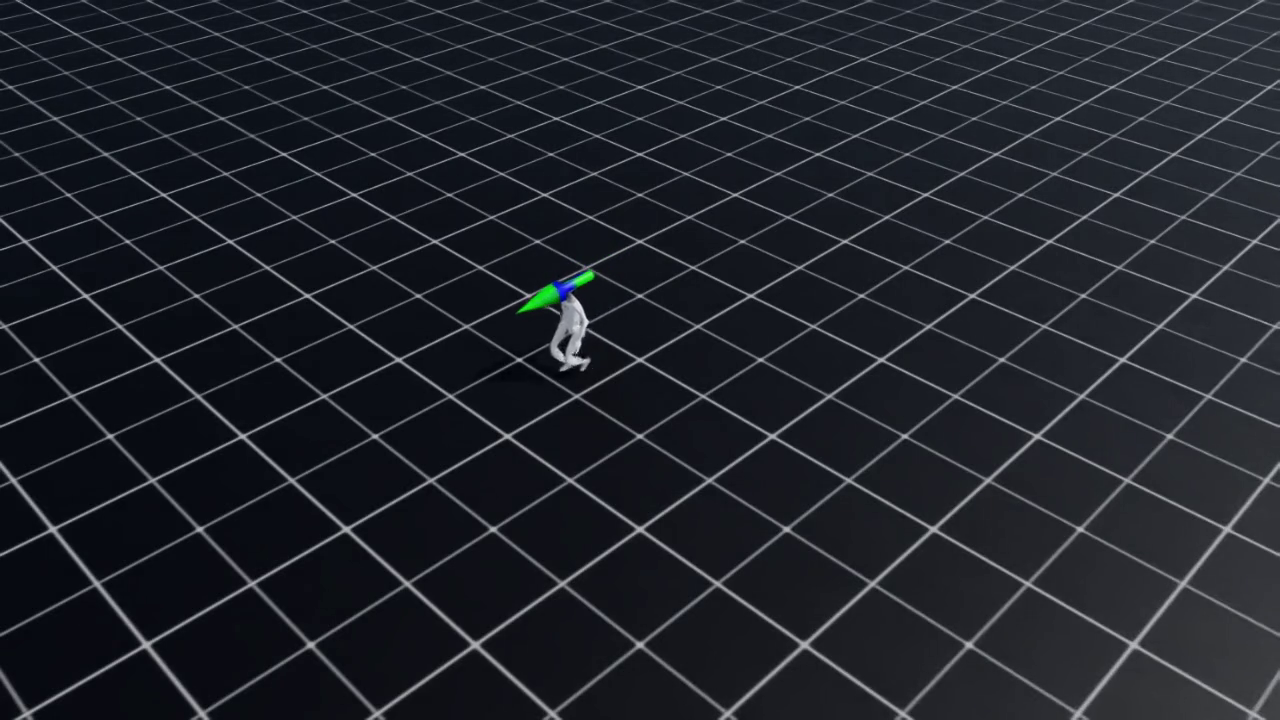
\includegraphics[width=\linewidth]{figures/fig_wide14.png}
\caption*{宽 $v_x$，$v_x{=}1.4\,\mathrm{m/s}$。}
\end{subfigure}
\hfill
\begin{subfigure}[t]{0.48\textwidth}
\centering
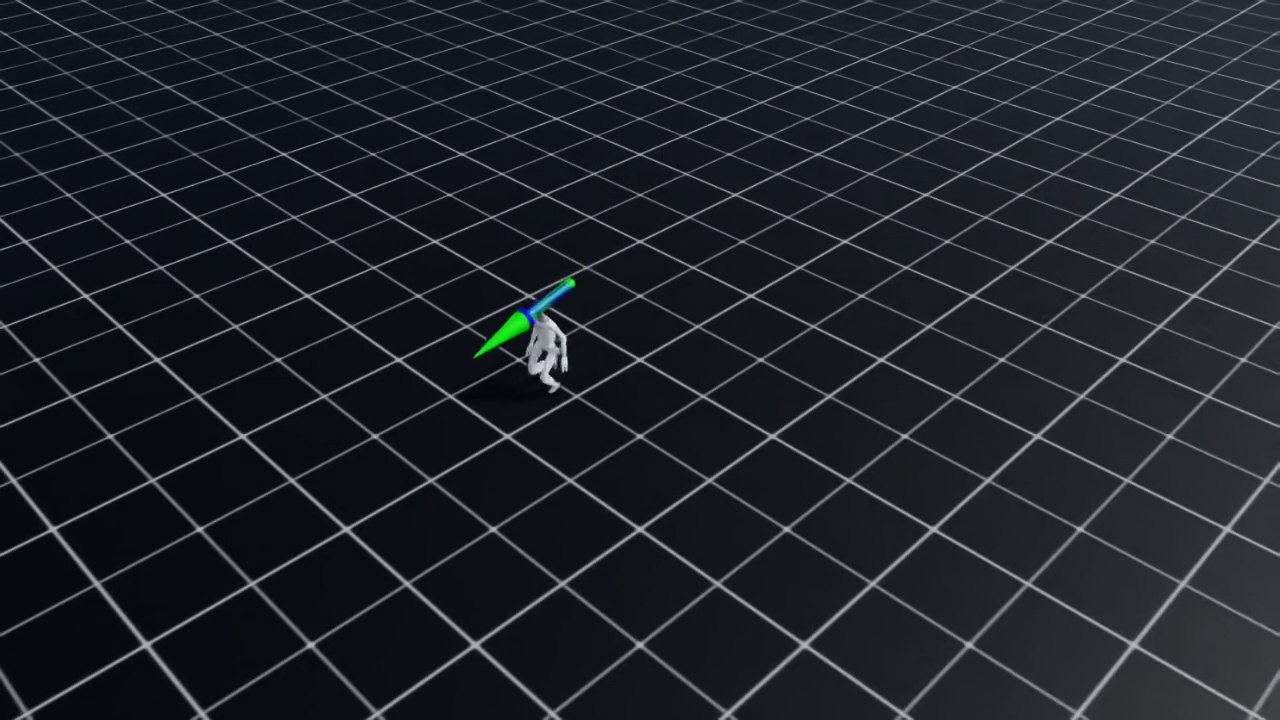
\includegraphics[width=\linewidth]{figures/fig_wide20.png}
\caption*{宽 $v_x$，$v_x{=}2.0\,\mathrm{m/s}$。}
\end{subfigure}
\caption{OOD 前进速度帧。基础策略在 $v_x{=}1.3\,\mathrm{m/s}$ 时保持，但在 $v_x{=}1.4\,\mathrm{m/s}$ 时倒下；宽 $v_x$ 在 $v_x{=}1.4\,\mathrm{m/s}$ 时恢复，并在 $v_x{=}2.0\,\mathrm{m/s}$ 时仍能行走。}
\label{fig:ood}
\end{figure}

\section{探索实验二：崎岖地形微调}
\label{sec:rough}

本实验考察平地 G1 速度策略能否在\textbf{不改变}观测维度的前提下迁移到不规则地面，
从而使预训练权重仍可兼容加载。

\subsection{动机}

官方崎岖地形（楼梯、随机箱子、高度噪声、斜坡）通常在策略观测中带有高度扫描仪。
平地策略无高度扫描（$123$ 维）。
启用扫描仪会改变网络输入尺寸，预训练检查点将无法加载。
能否在关闭高度扫描的情况下，仅对崎岖\textbf{物理}进行微调，仍获得可用的行走？

\subsection{设置}

\begin{table}[H]
\centering
\small
\begin{tabular}{@{}ll@{}}
\toprule
项目 & 选择 \\
\midrule
地形 & \texttt{ROUGH\_TERRAINS\_CFG} + 从 level~0 开始的课程 \\
观测 & 与平地相同：无 \texttt{height\_scan} \\
初始化 & 基础平地速度策略（非宽 $v_x$ 策略） \\
指令 & $v_x\in[0,2]$，$v_y\in[-0.5,0.5]$，$\omega_z\in[-1,1]$ \\
奖励 & 官方 G1 崎岖；\texttt{lin\_vel\_z\_l2}${}=0$ \\
环境数 & 4096 \\
\bottomrule
\end{tabular}
\caption{崎岖地形微调设置。}
\label{tab:rough}
\end{table}

微调从基础平地策略开始，因此同时将前进指令范围扩大到 $[0,2]\,\mathrm{m/s}$ 并更换地形。
竖直速度惩罚 \texttt{lin\_vel\_z\_l2} 设为零，因为上下楼梯需要基座竖直运动，
平地奖励会对此加以惩罚。

\subsection{训练}

平地策略在崎岖地形上微调 351 次迭代。
图~\ref{fig:tb-rough} 显示平均 episode 长度上升并稳定在约 $850$ 个控制步附近，
同时地形课程从 level~$1$ 升至约 $3.4$。

\begin{figure}[H]
\centering
\begin{subfigure}[t]{0.48\textwidth}
\centering
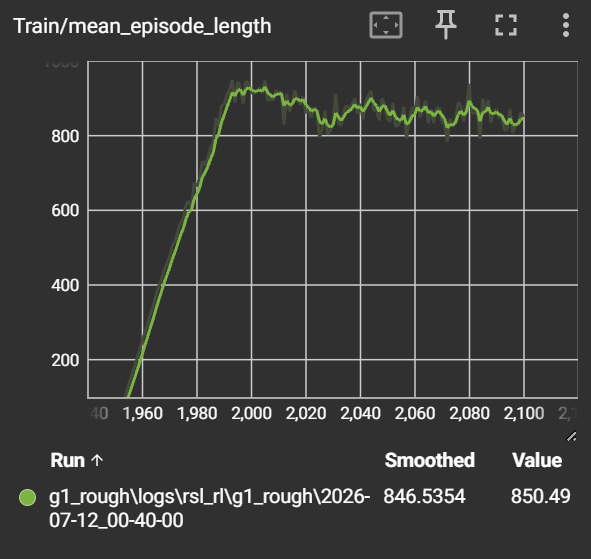
\includegraphics[width=\linewidth]{figures/tb_g1_rough_eps_length.png}
\caption*{平均 episode 长度。}
\end{subfigure}
\hfill
\begin{subfigure}[t]{0.48\textwidth}
\centering
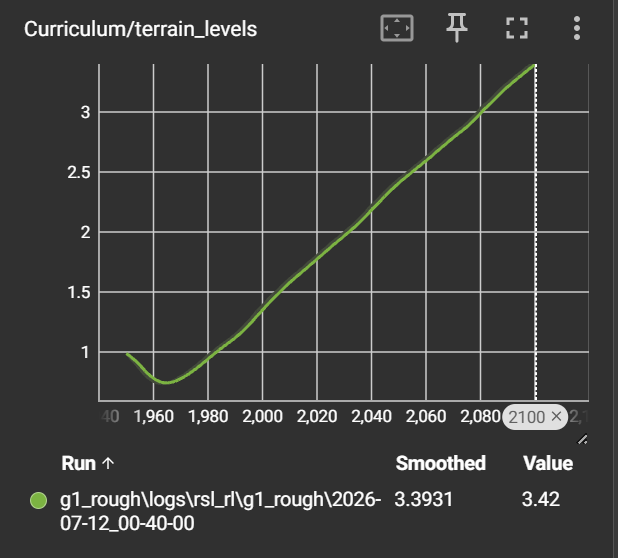
\includegraphics[width=\linewidth]{figures/tb_g1_rough_terrain_levels.png}
\caption*{地形课程等级。}
\end{subfigure}
\caption{崎岖地形微调：episode 长度与课程进度。}
\label{fig:tb-rough}
\end{figure}

\subsection{结果}

微调后，策略可在无高度扫描的情况下走过楼梯、随机箱子、斜坡与高度噪声。
在部分更难的地块上仍会跌倒，因为它无法预知前方地形，只能在接触后作出反应。
更多训练或许有帮助，但 GPU 当时另有安排。

\begin{figure}[H]
\centering
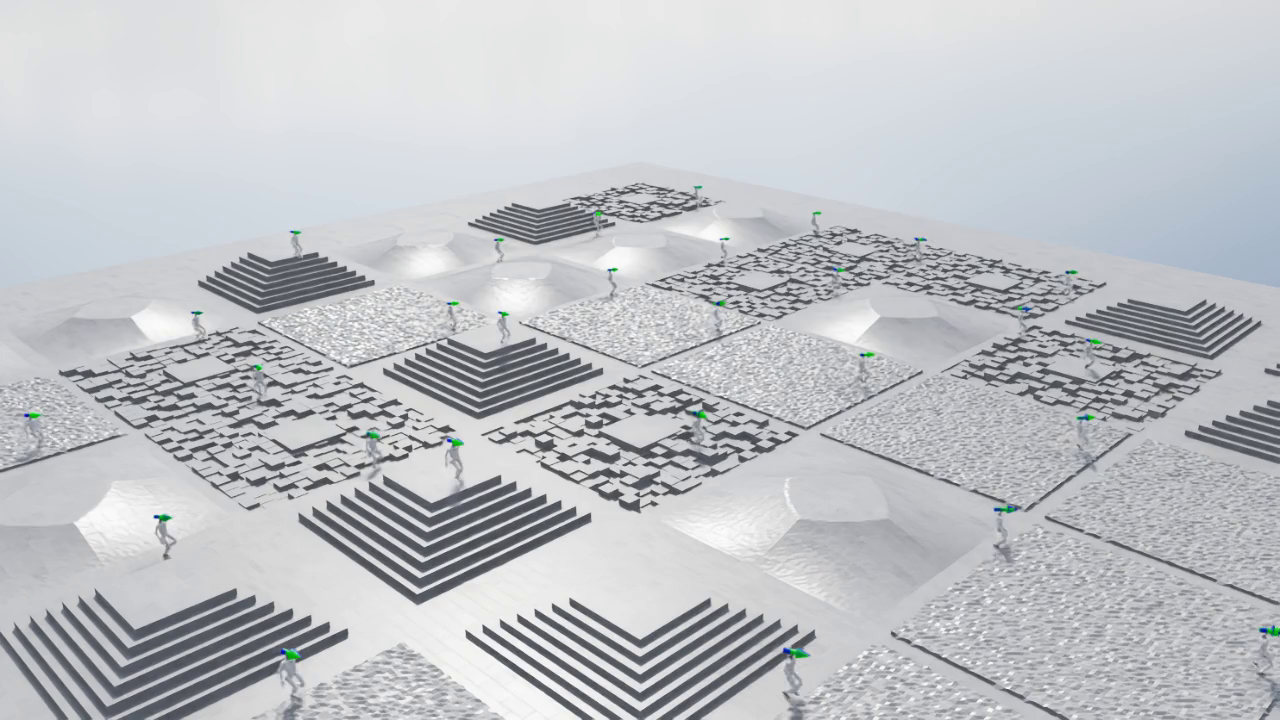
\includegraphics[width=0.92\textwidth]{figures/fig_rough.png}
\caption{微调后的崎岖地形演示。策略在无高度扫描的情况下穿越楼梯、随机箱子、高度噪声与斜坡。}
\label{fig:rough}
\end{figure}

\section{总结}
\label{sec:summary}

主要结论是：速度策略可复用于目标跟踪——简单的比例控制器生成速度指令，
学习到的策略负责行走。实验也表明训练分布至关重要。微调将所测前进速度从
$1.3\,\mathrm{m/s}$ 扩展到 $2.0\,\mathrm{m/s}$，并使平地策略在不改变观测尺寸的
情况下能在崎岖地形上行走。

主要局限在于：速度与崎岖地形结果基于定性视频，而非重复试验或数值基准。
崎岖策略仅短暂微调且无高度扫描，因而无法看见前方地形。我仅在仿真中评估策略。

\bibliographystyle{plainnat}
\bibliography{ref}
\end{document}
